%
% File: chap01.tex
% Author: Victor F. Brena-Medina
% Description: Introduction chapter where the biology goes.
%
\let\textcircled=\pgftextcircled
\chapter{The 8T-Static RAM}
\label{chap:sram_about}
%\paragraph{}

\section{Overview}

\paragraph{}
In this chapter we will discuss about the 8T Static Random Access Memory and the reason for considering it over 6T SRAM. Also, the read and write stability of the memory cell will be discussed.

\section{The Memory Core}
\paragraph{}

The 8T SRAM memory cell in Figure 3.1 consists of two back to back inverters, which hold the bit and it's complement without loss of charge unlike DRAM. It has two NMOS pass transistors connected to the WBL(Write Bit Line) and WBLB(Write Bit Line Bar) lines to write into the memory cell. The complement bit drives the gate of the transistor M7 which in turn is connected to a NMOS pass transistor controlled by the RWL or Read Word Line command. This path is used to produce the value of bit stored in the cell on RBL(Read Bit Line).
\begin{figure}[H]
\centering
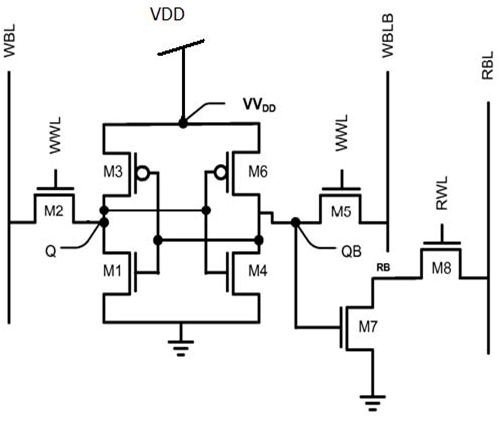
\includegraphics[width=0.6\textwidth]{chapters/chapter03/sram_actual1.png}
\caption{The 8T SRAM cell \emph{(Courtesy Google)}}
\label{fig:Figure}
\end{figure}

For the write operation the WBL is charged or discharged according to the bit that is to be stored and the WBLB is charged or discharged opposite of WBL. When the WWL(Write Word Line) signal is high, the NMOS pass transistor allows the path between the WBL, Q and WBLB and QB. When writing the cell with an opposite value stored inside the cell, it essential to keep in mind that to invert the bit value a charging or discharging at Q or QB must be stronger than the inverter's charging or discharging of the bit value. The sizing thus is done keeping in mind the write stability.

\begin{figure}[H]
\centering
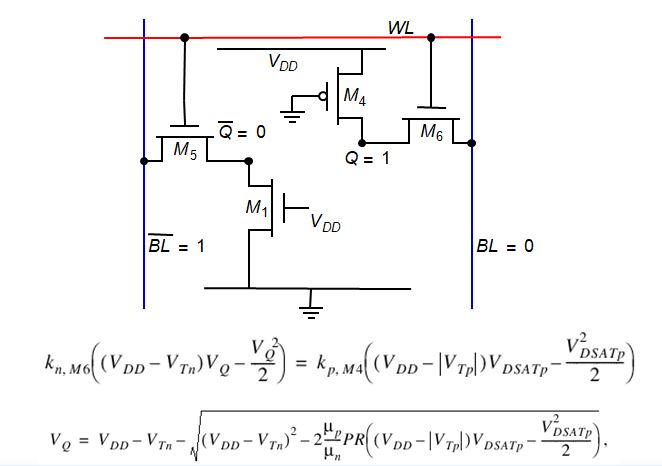
\includegraphics[width=0.6\textwidth]{writes.JPG}
\caption{Condition for writing the SRAM cell \emph{ (Chapter-12 Digital Integrated Circuits, Rabaey)}}
\label{fig:Figure}
\end{figure}

For the read operation the RBL is pre charged to VDD, when the M8 pass transistor is on and M7 is off the charge at RBL is retained which signifies bit 1 is stored, when M7 is on the charge is drained from RBL which signifies bit 0 is stored in the cell. The read operation is stable is stable and does not corrupt the the bit stored in the cell as QB is connected to the gate of the NMOS transistor.

\begin{figure}[H]
\centering
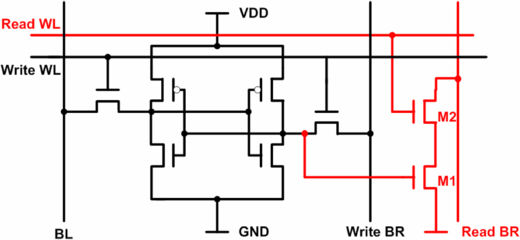
\includegraphics[width=0.7\textwidth]{readsram.jpg}
\caption{The Read path in 8T-SRAM cell \emph{(Courtesy Google)}}
\label{fig:Figure}
\end{figure}

\section{Why not 6T?}
\paragraph{}

As we just saw, that the 8T SRAM cell has decoupled read and write ports, thus there is very high read stability while reading from the cell. In contrast to 8T, the widely popular and more compact 6T SRAM cell does not have a read port separately as seen in Figure 3.3(b). The write and read operations occur from the same pass transistors. The sizing is hence done such that the read operation does not corrupt the stored bit, as the bit line is pre-charged for the reading cycle. Also even after sizing, due to process variations there still can be chances or error while reading. 

Along with this factor, the decoupled read port allows for some optimizations in the design techniques in which the RBL can be simultaneously used for logical operations by activating two or more 8T SRAM cells in the same column[2] as well as a Voltage Divider[2] along with a skewed inverter which will be discussed in the further chapters.

\begin{figure}[h]
\begin{subfigure}{0.5\textwidth}
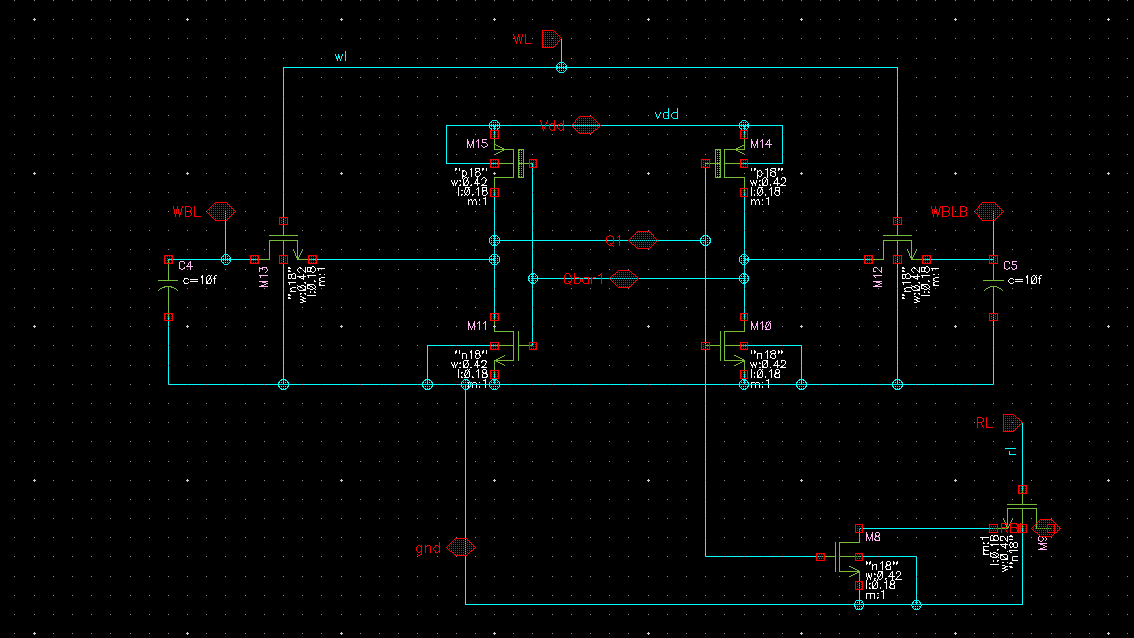
\includegraphics[width=0.9\linewidth, height = 0.7\linewidth]{chapters/chapter03/8t_sram_cell.png} 
\caption{the 8T SRAM Cell used in the project}
\label{fig:Figure}
\end{subfigure}
\begin{subfigure}{0.5\textwidth}
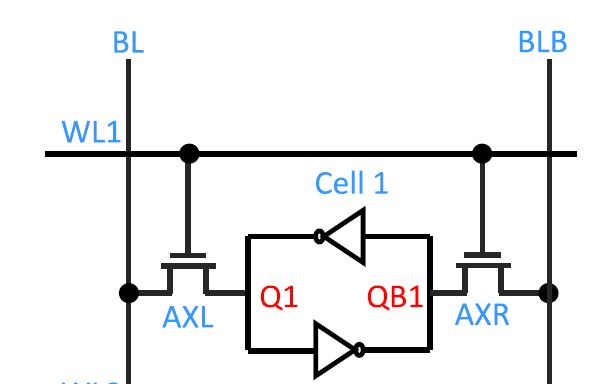
\includegraphics[width=0.9\linewidth, height = 0.7\linewidth]{6tsram.JPG}
\caption{The 6T SRAM cell[2]}
\label{fig:Figure}
\end{subfigure}
 
\caption{Comparison between 6T and 8T SRAM cells}
\label{fig:Figure}
\end{figure}




\section{Summary}

\paragraph{}
The reason for using 8T SRAM cells as the fundamental memory cell of the In-Memory Computation Architecture was justified. The inherently 'NOR wired' RBL when two or more 8T cells are activated will form the basis of designing logical operations without using gates. This optimization is discussed in detail in the next chapter. 